%\newgeometry{bottom=1cm,top=1cm}
\chapter{Filtri Passivi primo ordine}
\label{cha:Filtripassiviprimoord}
\begin{table}[t]
\centering
     \begin{minipage}{0.4\textwidth}
      \centering
       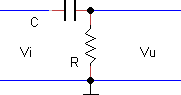
\includegraphics{extra/filtri/filtro_PA_CR}
\centering
 \begin{align*}
A&=\dfrac{V_{u}}{V_{i}}
=\dfrac{R}{R+\dfrac{1}{J2\pi fC}}=\\
&=\dfrac{J2\pi fRC}{1+J2\pi cfRC}=
\dfrac{1}{1+\dfrac{1}{J2\pi fRC}}\\
f_{c}&=\dfrac{1}{2\pi RC}
        \end{align*}
       \end{minipage}\hfill
\begin{minipage}[t]{0.4\textwidth}
      \centering
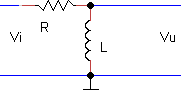
\includegraphics{extra/filtri/filtro_PA_RL}
\centering
     \begin{align*}
A&=\dfrac{V_{u}}{V_{i}}&=\dfrac{J2\pi fL}{R+J2\pi cfL}=\\
\dfrac{J2\pi f\dfrac{L}{R}}{1+J2\pi f\dfrac{L}{R}}
&=\dfrac{1}{1+\dfrac{1}{J2\pi f\dfrac{L}{R}}}\\
f_{c}&=\dfrac{1}{2\pi \dfrac{L}{R}}
        \end{align*}
     \end{minipage}
 \begin{subfigure}[b]{.5\linewidth}
 	\centering\includegraphics[scale=0.6]{extra/filtri/filtropa}
 	\caption{Filtro PA Grafico}
 \end{subfigure}
%\subfloat[][Filtro PA Grafico]{
%\centering
%  \includegraphics[scale=0.6]{filtropa}}
\caption{Filtro passa alto}
\label{tab:filtropassaalto}
\end{table}
\begin{table} %[htbp]
\centering
\begin{minipage}{0.4\textwidth}
      \centering
     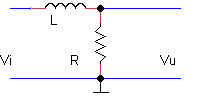
\includegraphics{extra/filtri/filtro_PB_LR}
\centering
 \begin{align*}
A&=\dfrac{V_{u}}{V_{i}}
=\dfrac{R}{R+J2\pi fL}\\
&=\dfrac{1}{1+J2\pi f\dfrac{L}{R}}\\
f_{c}&=\dfrac{1}{2\pi \dfrac{L}{R}}
        \end{align*} 
 \end{minipage}\hfill
  \begin{minipage}{0.4\textwidth}
      \centering
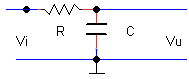
\includegraphics{extra/filtri/filtro_PB_RC}
  \centering
\begin{align*}
A&=\dfrac{V_{u}}{V_{i}}
=\dfrac{\dfrac{1}{J2\pi fc}}{R+\dfrac{1}{J2\pi fC}}=\\
&=\dfrac{1}{1+J2\pi fRC}\\
f_{c}&=\dfrac{1}{2\pi RC}
        \end{align*}
       %\caption{Passa Basso}
     \end{minipage}
  \begin{subfigure}[b]{.5\linewidth}
  	\centering\includegraphics[scale=0.6]{extra/filtri/filtropb}
  	\caption{Filtro PA Grafico}
  \end{subfigure}
%\subfloat[][Filtro PA Grafico]{
%\centering
%  \includegraphics[scale=0.6]{filtropb}}
\caption{Filtro passa basso}
\label{tab:filtropassabasso}
\end{table}


